Following up on the last part of the previous section, after composing the donut recipe in TableGen's syntax, it's time to print out a normal recipe from that via a custom-built TableGen backend.

\begin{tcolorbox}[colback=blue!5!white,colframe=blue!75!black, fonttitle=\bfseries,title=Note]
\hspace*{0.7cm}Please don't confuse a TableGen backend with a LLVM backend: the former converts (or transpiles) TableGen files into an arbitrary textual content, C/C++ header files being the most common form. An LLVM backend, on the other hand, lowers LLVM intermediate representations (IR) into low-level assembly code.
\end{tcolorbox}

In this section, we're developing the TableGen backend to print the donut we composed in the previous section into content, like this:

\begin{tcblisting}{commandshell={}}
=======Ingredients=======
1. oil 500 ml
2. flour 300 g
3. milk 1.25 cup
4. whole egg 1
5. yeast 1.50 tsp
6. butter 3.50 tbsp
7. sugar 2.0 tbsp
8. salt 0.50 tsp
9. vanilla extract 1.0 tsp

=======Instructions=======
1. use deep fryer to heat oil until 160 C
2. use mixer to mix flour, milk, whole egg, yeast, butter,
sugar, salt, and vanilla extract. stir in low speed.
3. use mixer to mix outcome from (step 2). stir in medium
speed.
4. use bowl to ferment outcome from (step 3).
5. use rolling pin to flatten outcome from (step 4).
6. use cutter to cut outcome from (step 5).
7. use deep fryer to fry outcome from (step 1) and outcome from
(step 6).
\end{tcblisting}

First, we will give an overview of llvm-tblgen, the program for driving the TableGen translation process. Then, we will show you how to develop our recipe-printing TableGen backend. Finally, we'll show you how to integrate our backend into the llvm-tblgen executable.


\subsubsubsection{4.4.1\hspace{0.2cm}TableGen's high-level workflow}

The TableGen backend takes in-memory representation (in the form of C++ objects) of the TableGen code we just learned and transforms it into arbitrary textual content. The whole process is driven by the llvm-tblgen executable, whose workflow can be illustrated by this diagram:

\hspace*{\fill} \\ %插入空行
\begin{center}
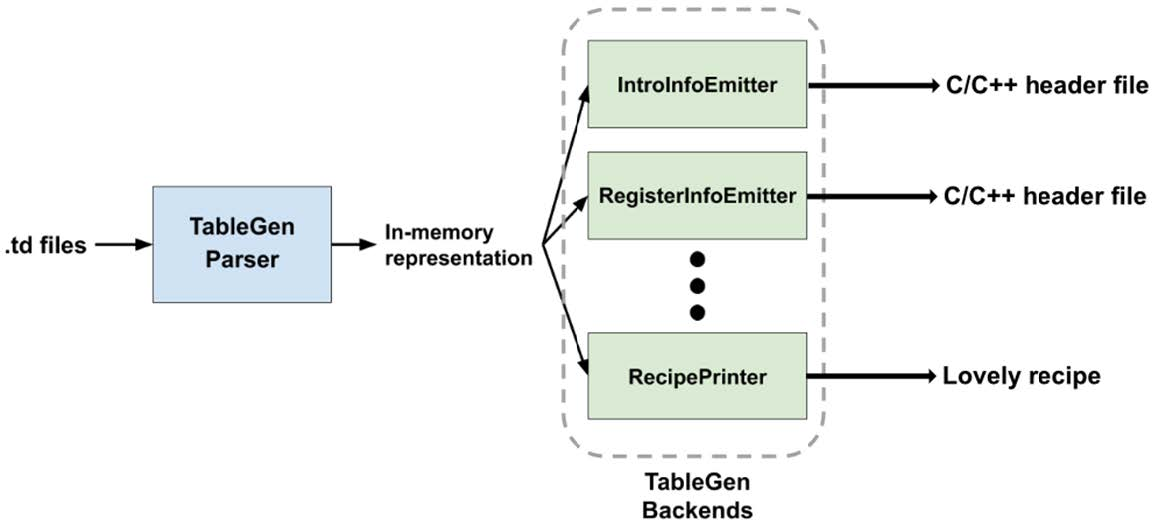
\includegraphics[width=0.9\textwidth]{content/1/chapter4/images/1.jpg}\\
Figure 4.1 – Workflow of llvm-tblgen
\end{center}

TableGen code's in-memory representation (which consists of C++ types and APIs) plays an important role in the TableGen backend development. Similar to LLVM IR, it is organized hierarchically. Starting from the top level, here is a list of its hierarchy, where each of the items is a C++ class:

\begin{itemize}
\item RecordKeeper: A collection (and owner) of all Record objects in the current translation unit.
\item Record: Represents a record or a class. The enclosing fields are represented by RecordVal. If it's a class, you can also access its template arguments.
\item RecordVal: Represents a pair of record fields and their initialized value, along with supplementary information such as the field's type and source location.
\item Init: Represents the initialized value of a field. It is a parent class of many, which represents different types of initialized values—For example, IntInit for integer values and DagInit for DAG values.
\end{itemize}

To give you a little task on the practical aspect of a TableGen backend, here is the skeleton of it:

\begin{lstlisting}[style=styleCXX]
class SampleEmitter {
	RecordKeeper &Records;
public:
	SampleEmitter(RecordKeeper &RK) : Records(RK) {}
	void run(raw_ostream &OS);
};
\end{lstlisting}

This emitter basically takes a RecordKeeper object (passed in by the constructor) as the input and prints the output into the raw\_ostream stream—the function argument of SampleEmitter::run.

In the next section, we're going to show you how to set up the development environment and get hands- on, writing a TableGen backend.

\subsubsubsection{4.4.2\hspace{0.2cm}Writing the TableGen backend}

In this section, we're showing you the steps of writing a backend to print out recipes written in TableGen. Let's start with the setup.

\hspace*{\fill} \\ %插入空行
\noindent
\textbf{Project setup}

To get started, LLVM has already provided a skeleton for writing a TableGen backend. So, please copy the llvm/lib/TableGen/TableGenBackendSkeleton.cpp file from the LLVM Project's source tree into the llvm/utils/TableGen folder, as follows:

\begin{tcblisting}{commandshell={}}
$ cd llvm
$ cp lib/TableGen/TableGenBackendSkeleton.cpp \
      utils/TableGen/RecipePrinter.cpp
\end{tcblisting}

Then, refactor the cSkeletonEmitter class into RecipePrinter.

RecipePrinter has the following workflow:

\begin{enumerate}
\item Collect all baking steps and ingredient records.
\item Print individual ingredients in textual formats using individual functions to print measuring units, temperature, equipment, and so on in textual formats.
\item Linearize the DAG of all baking steps.
\item Print each linearized baking step using a function to print custom formatting.
\end{enumerate}

We're not going to cover all the implementation details since lots of backend codes are actually not directly related to TableGen (text formatting and string processing, for example). Therefore, the following subsections only focus on how to retrieve information from TableGen's in-memory objects.

\hspace*{\fill} \\ %插入空行
\noindent
\textbf{Getting all the baking steps}

In the TableGen backend, a TableGen record is represented by the Record C++ class. When we want to retrieve all the records derived from a specific TableGen class, we can use one of the functions of RecordKeeper: getAllDerivedDefinitions. For instance, let's say we want to fetch all the baking steps records that derived from the Step TableGen class in this case. Here is how we do with getAllDerivedDefinitions:

\begin{lstlisting}[style=styleCXX]
// In RecipePrinter::run method…
std::vector<Record*> Steps = Records.
getAllDerivedDefinitions("Step");
\end{lstlisting}

This gives us a list of Record pointers that represent all of the Step records.

\begin{tcolorbox}[colback=blue!5!white,colframe=blue!75!black, fonttitle=\bfseries,title=Note]
\hspace*{0.7cm}For the rest of this section, we will use Record in this format (with Courier font face) to refer to the C++ counterpart of a TableGen record.
\end{tcolorbox}

\hspace*{\fill} \\ %插入空行
\noindent
\textbf{Retrieving field values}

Retrieving field values from Record is probably the most basic operation. Let's say we're working on a method for printing Unit record objects introduced earlier, as follows:

\begin{lstlisting}[style=styleCXX]
void RecipePrinter::printUnit(raw_ostream& OS, Record*
UnitRecord) {
	OS << UnitRecord->getValueAsString("Text");
}
\end{lstlisting}

The Record class provides some handy functions, such as getValueAsString, to retrieve the value of a field and try to convert it into a specific type so that you don't need to retrieve the RecordVal value of a specific field (in this case, the Text field) before getting the real value. Similar functions include the following:

\begin{itemize}
\tt
\item Record* getValueAsDef(StringRef FieldName)
\item bool getValueAsBit(StringRef FieldName)
\item int64\_t getValueAsInt(StringRef FieldName)
\item DagInit* getValueAsDag(StringRef FieldName)
\end{itemize}

In addition to these utility functions, we sometimes just want to check if a specific field exists in a record. In such cases, call Record::getValue(StringRef FieldName) and check if the returned value is null. But just be aware that not every field needs to be initialized; you may still need to check if a field exists, but is uninitialized. When that happens, let Record::isValueUnset help you.

\begin{tcolorbox}[colback=blue!5!white,colframe=blue!75!black, fonttitle=\bfseries,title=Note]
\hspace*{0.7cm}TableGen actually uses a special Init class, UnsetInit, to represent an uninitialized value.
\end{tcolorbox}

\hspace*{\fill} \\ %插入空行
\noindent
\textbf{Type conversion}

Init represents initialization values, but most of the time we're not directly working with it but with one of its children's classes.

For example, StepOrIngredient is an Init type object that represents either a Step record or an ingredient record. It would be easier for us to convert it to its underlying DefInit object since DefInit provides richer functionalities. We can use the following code to typecast the Init type StepOrIngredient into a DefInit type object:

\begin{lstlisting}[style=styleCXX]
const auto* SIDef = cast<const DefInit>(StepOrIngredient);
\end{lstlisting}

You can also use isa<…>(…) to check its underlying type first, or dyn\_cast<…>(…) if you don't want to receive an exception when the conversion fails.

Record represents a TableGen record, but it would be better if we can find out its parent class, which further tells us the field's information.

For example, after getting the underlying Record object for SIDef, we can use the isSubClassOf function to tell if that Record is a baking step or ingredient, as follows:

\begin{lstlisting}[style=styleCXX]
Record* SIRecord = SIDef->getDef();
if (SIRecord->isSubClassOf("Step")) {
	// This Record is a baking step!
} else if (SIRecord->isSubClassOf("IngredientBase")){
	// This Record is an ingredient!
}
\end{lstlisting}

Knowing what the underlying TableGen class actually is can help us to print that record in its own way.

\hspace*{\fill} \\ %插入空行
\noindent
\textbf{Handling DAG values}

Now, we are going to print out the Step records. Recall that we used the dag type to represent the action and the ingredients required for a baking step. Have a look at the following code example:

\begin{lstlisting}[style=styleCXX]
def step_prep : Step<(heat:$action fry_oil:$oil, oil_
temp:$temp)> {
	let CustomFormat = "$action $oil until $temp";
}
\end{lstlisting}

Here, the highlighted dag is stored in the Action field of the Step TableGen class. So, we use getValueAsDag to retrieve that field as a DagInit object, as follows:

\begin{lstlisting}[style=styleCXX]
DagInit* DAG = StepRecord->getValueAsDag("Action");
\end{lstlisting}

DagInit is just another class derived from Init, which wasintroduced earlier. It contains some DAG-specific APIs. For example, we can iterate through all of its operands and get their associated Init object using the getArg function, as follows:

\begin{lstlisting}[style=styleCXX]
for(i = 0; i < DAG->arg_size; ++i) {
	Init* Arg = DAG->getArg(i);
}
\end{lstlisting}

Furthermore, we can use the getArgNameStr function to retrieve the token (if there is any), which is always represented in string type in the TableGen backend, associated with a specific operand, as illustrated in the following code snippet:

\begin{lstlisting}[style=styleCXX]
for(i = 0; i < DAG->arg_size; ++i) {
	StringRef ArgTok = DAG->getArgNameStr(i);
}
\end{lstlisting}

If ArgTok is empty, this means there is no token associated with that operand. To get the token associated with the operator, we can use the getNameStr API.

\begin{tcolorbox}[colback=blue!5!white,colframe=blue!75!black, fonttitle=\bfseries,title=Note]
\hspace*{0.7cm}Both DagInit::getArgNameStr and DagInit::getNameStr return the token string without the leading dollar sign.
\end{tcolorbox}

This section has shown you some of the most important aspects of working with TableGen directives' in-memory C++ representation, which is the building block of writing a TableGen backend. In the next section, we will show you the final step to put everything together and run our custom TableGen backend.

\subsubsubsection{4.4.3\hspace{0.2cm}Integrating the RecipePrinter TableGen backend}

After finishing the utils/TableGen/RecipePrinter.cpp file, it's time to put everything together.

As mentioned before, a TableGen backend is always associated with the llvm-tblgen tool, which is also the only interface to use the backend. llvm-tblgen uses simple command-line options to choose a backend to use.

Here is an example of choosing one of the backends, IntrInfoEmitter, to generate a C/C++ header file from a TableGen file  that carries instruction set information of X86:

\begin{tcblisting}{commandshell={}}
$ llvm-tblgen -gen-instr-info /path/to/X86.td -o GenX86InstrInfo.inc
\end{tcblisting}

Let's now see how to integrate RecipePrinter source file to TableGen backend:

\begin{itemize}
\item To link the RecipePrinter source file into llvm-tblgen and add a command-line option to select it, we're going to use utils/TableGen/TableGenBackends.h first. This file only contains a list of TableGen backend entry functions, which are functions that take a raw\_ostream output stream and the RecordKeeper object as arguments. We're also putting our EmitRecipe function into the list, as follows:

\begin{lstlisting}[style=styleCXX]
…
void EmitX86FoldTables(RecordKeeper &RK, raw_ostream
&OS);
void EmitRecipe(RecordKeeper &RK, raw_ostream &OS);
void EmitRegisterBank(RecordKeeper &RK, raw_ostream &OS);
…
\end{lstlisting}

\item Next, inside llvm/utils/TableGen/TableGen.cpp, we're first adding a new ActionType enum element and the selected command-line option, as follows:

\begin{lstlisting}[style=styleCXX]
enum Action Type {
	…
	GenRecipe,
	… 
} 
…
cl::opt<ActionType> Action(
	cl::desc("Action to perform:"),
	cl::values(
		…
		clEnumValN(GenRecipe, "gen-recipe",
				   "Print delicious recipes"),
		…
	));
\end{lstlisting}

\item After that, go to the LLVMTableGenMain function and insert the function call to EmitRecipe, as follows:

\begin{lstlisting}[style=styleCXX]
bool LLVMTableGenMain(raw_ostream &OS, RecordKeeper
&Records) {
	switch (Action) {
		…
		case GenRecipe:
		EmitRecipe(Records, OS);
		break;
	}
}
\end{lstlisting}

\item Finally, don't forget to update utils/TableGen/CMakeLists.txt, as follows:

\begin{lstlisting}[style=styleCXX]
add_tablegen(llvm-tblgen LLVM
	…
	RecipePrinter.cpp
	…)
\end{lstlisting}

\item That's all there is to it! You can now run the following command:

\begin{tcblisting}{commandshell={}}
$ llvm-tblgen -gen-recipe DonutRecipe.td
\end{tcblisting}

(You can optionally redirect the output to a file using the -o option.)

The preceding command will print out a (mostly) normal donut recipe, just like this:

\begin{tcblisting}{commandshell={}}
=======Ingredients=======
1. oil 500 ml
2. flour 300 g
3. milk 1.25 cup
4. whole egg 1
5. yeast 1.50 tsp
6. butter 3.50 tbsp
7. sugar 2.0 tbsp
8. salt 0.50 tsp
9. vanilla extract 1.0 tsp

=======Instructions=======
1. use deep fryer to heat oil until 160 C
2. use mixer to mix flour, milk, whole egg, yeast,
butter, sugar, salt, and vanilla extract. stir in low
speed.
3. use mixer to mix outcome from (step 2). stir in medium
speed.
4. use bowl to ferment outcome from (step 3).
5. use rolling pin to flatten outcome from (step 4).
6. use cutter to cut outcome from (step 5).
7. use deep fryer to fry outcome from (step 1) and
outcome from (step 6).
\end{tcblisting}

\end{itemize}

In this section, we have learned how to build a custom TableGen backend to transform a recipe written in TableGen into normal plaintext format. Things we learned here include how llvm-tblgen, the driver of translating TableGen code, works; how to use the TableGen backend's C++ APIs to operate TableGen directive's in-memory representation; and how to integrate our custom backend into llvm-tblgen in order to run it. Combining the skills you learned in this chapter and in the previous one, you can create a complete and standalone toolchain that implements your custom logic, using TableGen as a solution.













































